
%(BEGIN_QUESTION)
% Copyright 2010, Tony R. Kuphaldt, released under the Creative Commons Attribution License (v 1.0)
% This means you may do almost anything with this work of mine, so long as you give me proper credit

Determine the approximate value of the {\it derivative} ($dy \over dx$) for this function where $x=2.5$:

$$\includegraphics[width=15.5cm]{i04366x01.eps}$$

Choose the closest answer:

\begin{itemize}
\item{} $dy \over dx$ = +3
\vskip 10pt 
\item{} $dy \over dx$ = $-3$
\vskip 10pt 
\item{} $dy \over dx$ = $-9$
\vskip 10pt 
\item{} $dy \over dx$ = $-2$
\vskip 10pt 
\item{} $dy \over dx$ = +2
\vskip 10pt 
\item{} $dy \over dx$ = 0
\vskip 10pt 
\item{} $dy \over dx$ = +1
\end{itemize}

\underbar{file i04366}
%(END_QUESTION)





%(BEGIN_ANSWER)

$dy \over dx$ = +2

%(END_ANSWER)





%(BEGIN_NOTES)


%INDEX% Mathematics, calculus: derivative (approximating derivative values at points on graph)

%(END_NOTES)


